\chapter{Introduction}

\section{Human Genetics and the Genetics of Complex Traits}

A central goal of genetics is to understand the contribution of genetic variation to phenotypic variation. 


\begin{figure}
\centering
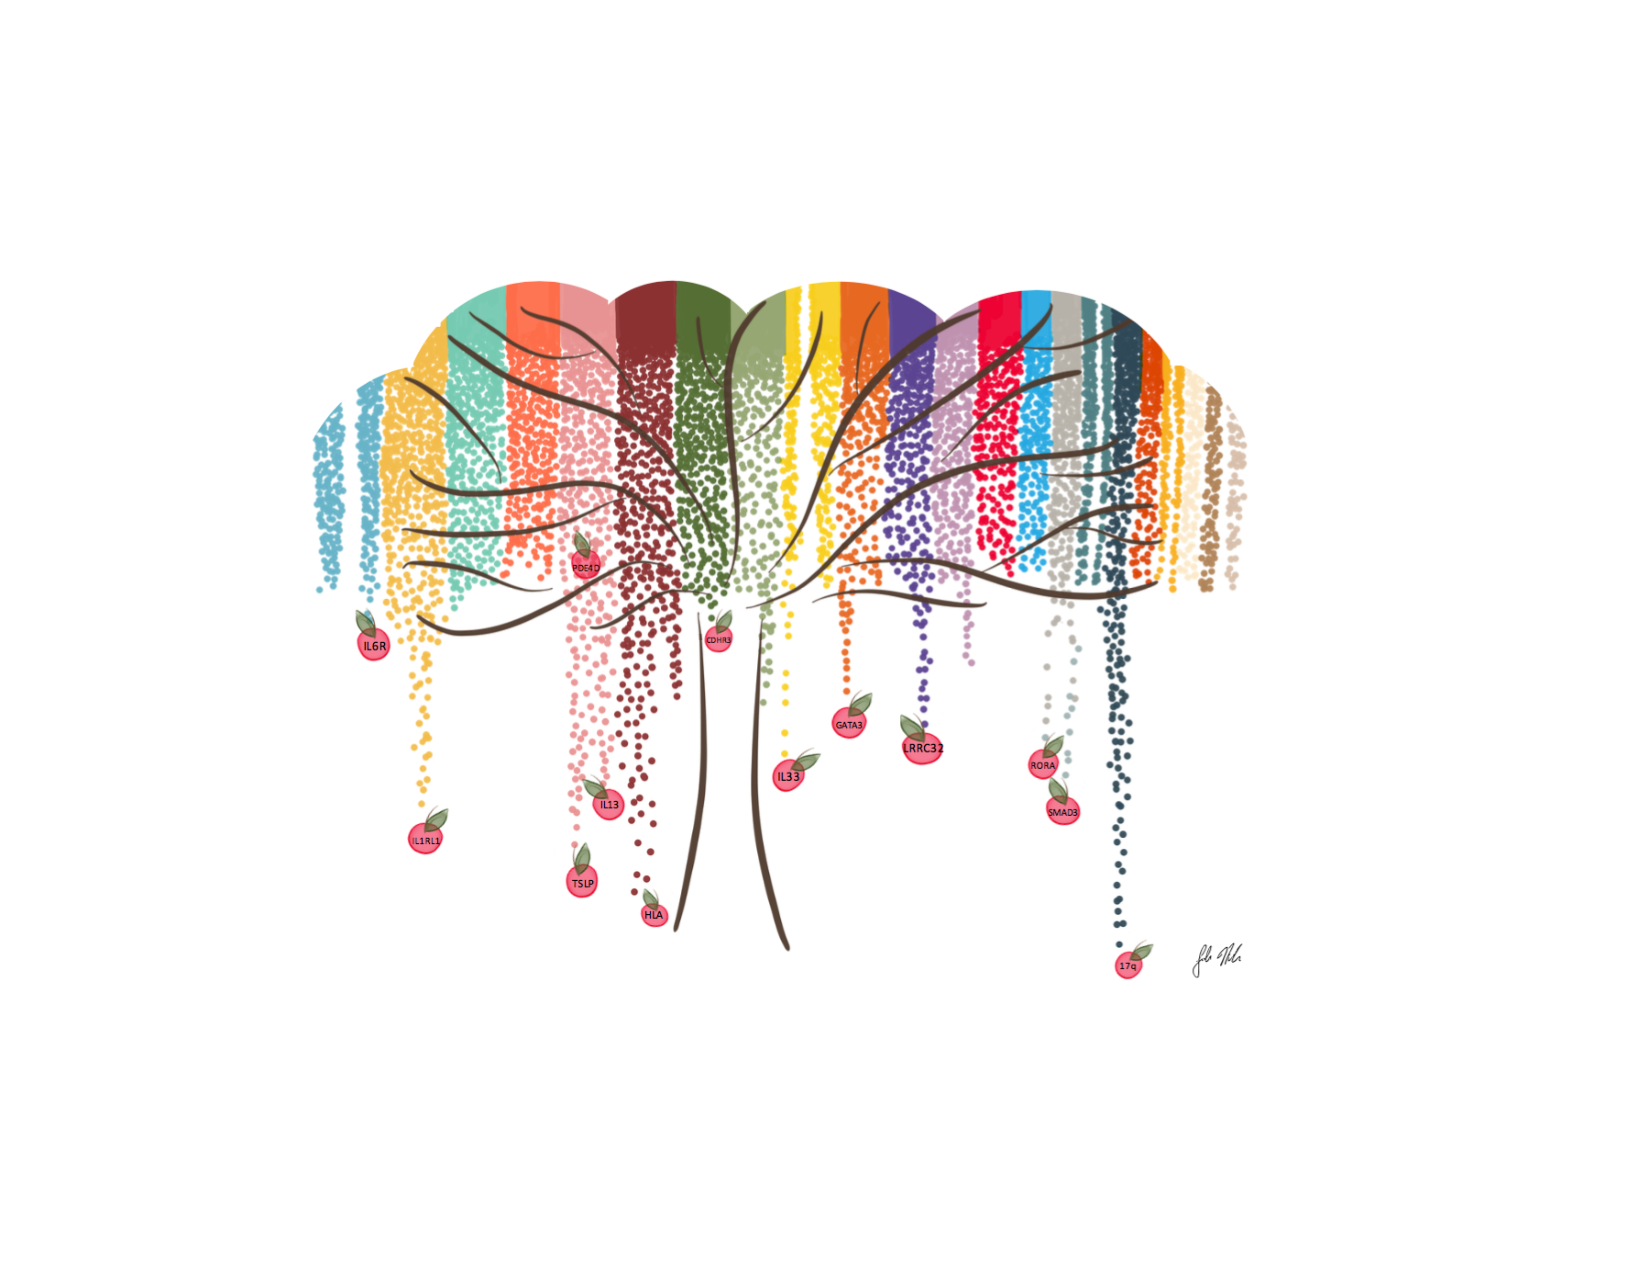
\includegraphics[width=8in]{img/ch01/fig-01-lowhangingfruit.pdf}
\caption[Low Hanging Fruit.]{\textbf{Asthma GWAS - low hanging fruit}}
\label{fig:lowhangingfruit}
\end{figure}


\section{The Origin of Genomic Imprinting }

Genomic imprinting in its broadest sense suggests that a phenotype observed for a particular gene or genes depends on the sex of the parent from with the gamete containing that gene or genes originated\cite{Sapienza:1989vm}. It was said that a particular gene is imprinted if it results in a different phenotype when it is maternally inherited versus paternally inherited.

The first use of the term "imprinting" was used in reference to the recognition by the cell of of chromosomes in \textit{Sciara}\cite{Crouse:1960vc,Sapienza:1989vm}. "The "imprint" a chromosome bears is unrelated to the genic constitution of the chromosome and is determined only by the sex of the germ line through with the chromosome has been inherited."\cite{Crouse:1960vc} 

The preferential inactivation of the paternally-derived X chromosomes in mouse were the first demonstrations of a functional imprint in mammalian genomes\cite{Takagi:1975ua,Lyon:1984gh,Chandra:1975tb}. The first suggestion of imprinting on autosomes was by a deletion on mouse chromosome 17 that showed a different phenotype based on which parent the deletion was inherited from.\cite{Johnson:1974uf,Johnson:1974kc}.

It was not until the development of the pronuclear transplantation technique that allowed for the creation of mice zygotes which contained only maternal or only paternal genetic contributions and provided evidence that the maternal and paternal genomes are not equal. The differential imprinting on the parental chromosomes prevented complete embryonic development in these mice with complete uniparental disomy.\cite{Sapienza:1989vm,McGrath:1984ky}.



\section{The Search for Parent of Origin Effects}


